\documentclass[a4paper, 14pt]{extarticle}
\usepackage{../generalPreamble}
\usepackage{../reportFormat}

\DeclareMathOperator{\floor}{floor}

% chktex-file 29

\begin{document}
\begin{titlepage}
    \centering
    {\bfseries
        \uppercase{
            Минобрнауки России \\
            Санкт-Петербургский государственный \\
            Электротехнический университет \\
            \enquote{ЛЭТИ} им. В.И.Ульянова (Ленина)\\
        }
        Кафедра ИБ

        \vspace{\fill}
        \uppercase{Отчёт} \\
        по лабораторной работе №6 \\
        по дисциплине \enquote{Криптография и защита информации} \\
        Тема: Изучение хэш-функций
    }

    \vspace{\fill}
    \begin{tabularx}{0.8\textwidth}{l X c r}
        Студент гр. 6304 & & \underline{\hspace{3cm}} & Корытов П.В.\\
        Преподаватель & & \underline{\hspace{3cm}} & Племянников А.К.
    \end{tabularx}

    \vspace{1cm}
    Санкт-Петербург \\
    \the\year{}
\end{titlepage}

\section*{Цель работы}
Исследование хэш-функций MD5, SHA-256, SHA-512, SHA-3, кода контроля целостности HMAC и анализ атак дополнительной коллизии на хэш-функцию. Получить практические навыки работы с хэш- функциями и атакой на них, в том числе и в программном продукте Cryptool 1 и 2.

\section{Исследование лавинного эффекта MD5, SHA-1, SHA-256, SHA-512}
\subsection{Описание алгоритмов}
\subsubsection{MD5}
MD5 перерабатывает сообщение произвольной длины в сообщение длины $128$ бит.

Сообщение дополняется, чтобы длина делилась на $512$
\begin{itemize}
    \item Добавляется бит 1
    \item Дописываются нули, чтобы осталось 64 бита
    \item В последние 64 бита записывается длина сообщения по модулю $2^{64}$\\
\end{itemize}

После чего сообщение делится на блоки по $512$ бит. Для каждого блока выполняет 4 раунда по 16 операций.

Структура одной операции MD5 представлена на рис.~\ref{img:md5}

\begin{figure}[h]
    \centering
    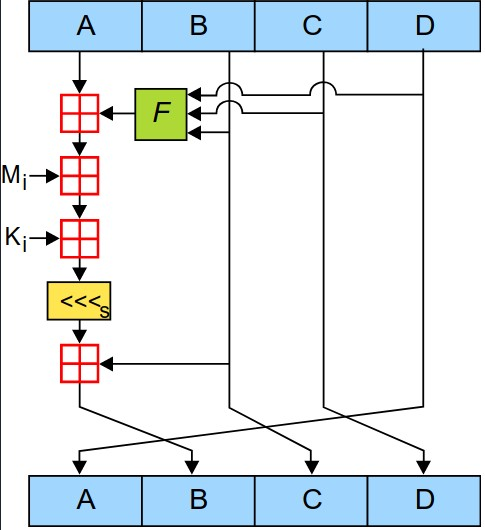
\includegraphics[width=0.5\textwidth]{img/S001.jpg}
    \caption{Одна операция MD5}%
    \label{img:md5}
\end{figure}

\FloatBarrier{}

MD5 оперирует на $128$-битном состоянии, поделённом на 4 слова по $32$ бит. 
\begin{itemize}
    \item Инициализация для 1-го блока:
    \begin{itemize}
        \item $A := 0x67452301$
        \item $B := 0xefcdab89$
        \item $ C:= 0x98badcfe $
        \item $D := 0x10325476$
    \end{itemize}
    \item $F$ --- нелинейная функция:
    \begin{equation}
        F(B,C,D) = \begin{cases}
            (B \wedge C) \vee (\neg B \wedge D), &\text{ если } i \in [0, 15]\\
            (B \wedge D) \vee (C \wedge \neg D), &\text{ если } i \in [16, 31]\\
            B \oplus C \oplus D, &\text{ если } i \in [32, 47]\\
            C \oplus (B \vee \neg D) &\text{ если } i \in [48, 63]\\
        \end{cases}
    \end{equation}
    \item $M_i$ --- часть входного блока размером $32$ бит. Выбор номера блока:
    \begin{equation}
        \begin{cases}
            i, &\text{ если } i \in [0, 15]\\
            (5i + 1) \bmod 16, &\text{ если } i \in [16, 31]\\
            (3i + 5) \bmod 16 &\text{ если } i \in [32, 47]\\
            7i \bmod 16 &\text{ если } i \\
        \end{cases}
    \end{equation}
    \item $K_i$ --- константа такого же размера, разная для каждой операции
    \begin{equation}
        K_i = \floor (2^{32} \bullet |\sin(i+1)|)
    \end{equation}
    \item ${<<<}_s$ --- сдвиг влево на $s$ бит
    \begin{itemize}
        \item $s[0, 15] = \{7, 12, 17, 22,  7, 12, 17, 22,  7, 12, 17, 22,  7, 12, 17, 22\}$
        \item $s[16, 31] = \{ 5,  9, 14, 20,  5,  9, 14, 20,  5,  9, 14, 20,  5,  9, 14, 20 \}$
        \item $s[32, 47] = \{ 4, 11, 16, 23,  4, 11, 16, 23,  4, 11, 16, 23,  4, 11, 16, 23 \} $
        \item $s[48, 63] = \{ 6, 10, 15, 21,  6, 10, 15, 21,  6, 10, 15, 21,  6, 10, 15, 21 \}$
    \end{itemize}
    \item $\boxplus$ --- сложение по модулю $2^{32}$\\
\end{itemize}

\subsubsection{SHA-1}
Длина хэша SHA-1 --- $160$ бит. Размер блока --- $512$ бит.

Размер блоков и правила дополнения совпадают с таковыми для MD5. Вид одной операции представлен на рис.~\ref{img:sha1}
\begin{figure}[h]
    \centering
    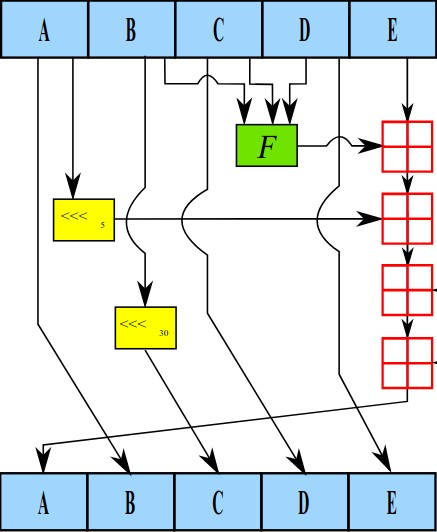
\includegraphics[width=0.5\textwidth]{img/S002.jpg}
    \caption{Одна итерация SHA-1}%
    \label{img:sha1}
\end{figure}

\FloatBarrier{}

\begin{itemize}
    \item Инициализация:
        \begin{itemize}
            \item $h0 = \mathtt{0x67452301}$
            \item $h1 = \mathtt{0xefcdab89}$
            \item $h2 = \mathtt{0x98badcfe}$
            \item $h3 = \mathtt{0x10325476}$
            \item $h4 = \mathtt{0xc3d2e1f0}$
    \end{itemize}
    \item $W_i$ --- расширение $16$ $32$-х слов входного блока до $80$. Для $i > 15$:
    \begin{equation}
        W_i = (W_{i-3} \oplus W_{i-8} \oplus W_{i-14} \oplus W_{i-16}) \lll 1
    \end{equation}
    \item $F$ такая же, как в MD5, но с промежутками по $20$ вместо $16$
    \item $K_i$ --- константа:
    \begin{equation}
        K = \begin{cases}
            \mathtt{0x5A827999} , &\text{ если } i \in [0, 19]\\
            \mathtt{0x6ED9EBA1} , &\text{ если } i \in [20, 39]\\
            \mathtt{0x8F1BBCDC} , &\text{ если } i \in [40, 59]\\
            \mathtt{0xCA62C1D6} , &\text{ если } i \in [60, 79]\\
        \end{cases}
    \end{equation}
\end{itemize}

\subsection{Формулировка задания}
\begin{itemize}
    \item  Открыть текст не менее 1000 знаков. Добавить свое ФИО последней строкой. Перейти к утилите Indiv.Procedures->Hash->Hash Demonstration..
    \item  Задать хэш-функцию, подлежащую исследованию: MD5, SHA-1, SHA-256, SHA-512.
    \item  Для каждой хэш-функции повторить следующие действия:
    \begin{itemize}
        \item  Измените (добавлением, заменой, удалением символа) исходный файл
        \item  Зафиксировать количество измененных битов в дайджесте модифицированного сообщения.
        \item  Вернуть сообщение в исходное состояние.
    \end{itemize}
    \item  Выполните процедуру 3 раза (добавлением, заменой, удалением символа) и подсчитайте среднее количество измененных бит дайджеста.  Зафиксировать результаты в таблице.
\end{itemize}

\subsection{Ход работы}
\lipsum[1] %TODO

\section{Хэш-функция SHA-3}
\subsection{Описание алгоритма}
SHA-3 построен на основе криптографической губки. Вид этой структуры представлен на рис.~\ref{img:sponge}

\begin{figure}[h]
    \centering
    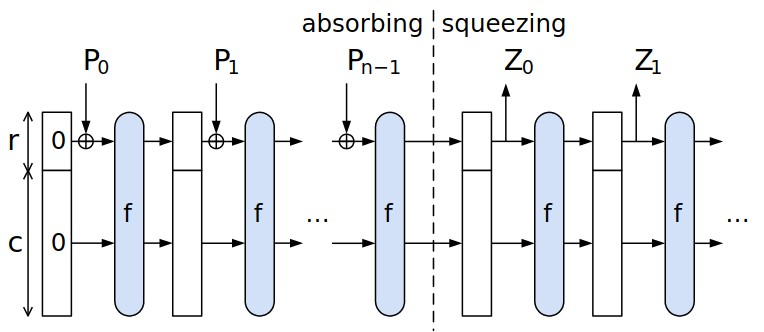
\includegraphics[width=0.8\textwidth]{img/S003.jpg}
    \caption{Губка}%
    \label{img:sponge}
\end{figure}

\FloatBarrier{}
\subsubsection{Дополнение}
Сообщение должно быть поделено на блоки по $r$ бит. Для этого к сообщению добавляется блок вида $10\ldots01$.

Если последний блок имеет длину $r-1$, то он дополняется единицей, следующий блок состоит из $r-1$ нулей и $1$.

Если длина последнего блока $r$, то все равно добавляется блок описанного вида.

\subsubsection{Устройство губки}
На входе:
\begin{itemize}
    \item $P$ разбивается на блоки $P_0, \ldots, P_{n-1}$ по $r$ бит
    \item Инциализация $S$ нулевым вектором
    \item Впитывание (Absorbing):
        \begin{itemize}
            \item $P_i$ дополняется $c$ нулями до длины блока $b$
            \item Это побитово складывается с $S$
            \item Состояние модифицируется функцией $f$
        \end{itemize}
    \item Отжатие (Squeezing)\\
    На каждом шаге от $S$ сохраняются первые $r$ байт, после чего применяется $f$. Так повторяется, пока не получится выход $Z$ новой длины

\end{itemize}

\subsection{Формулировка задания}
\begin{itemize}
    \item  Открыть шаблон Keccak Hash (SHA-3) в Cryptool 2
    \item  В модуле Keccak сделать следующие настройки:
    \begin{itemize}
        \item  Adjust manually=ON
        \item  Keccak version= SHA3--512
    \end{itemize}
    \item  Загрузить файл из предыдущего задания
    \item  Запустить проигрывание шаблона в режиме ручного управления:
    \begin{itemize}
        \item  Сохранить скриншоты преобразований первого раунда
        \item  Сохранить скриншот заключительной фазы
        \item  Сохранить значение дайджеста
    \end{itemize}
    \item  Вычислить значения дайджеста для модифицированных текстов из предыдущего задания
    \item  Подсчитать лавинный эффект с помощью самостоятельно разработанной автоматизированной процедуры
\end{itemize}

\subsection{Ход работы}
\lipsum[1] %TODO

\section{Контроль целостности по коду HMAC}
\subsection{Описание механизма}
HMAC позволяет контролировать целостность данных, передаваемых в ненадежной среде. Два клиента разделяют общий секретный ключ.
\begin{equation}
    HMAC_k(\mathtt{text}) = H((K \oplus \mathtt{opad}) || H ((K \oplus \mathtt{ipad}) || \mathtt{text}) ),
\end{equation}
где:
\begin{itemize}
    \item $||$ --- конкатенация;
    \item $K$ --- секретный ключ;
    \item \texttt{ipad} --- блок, где байт \texttt{0x36} повторяется $b$ раз;
    \item \texttt{opad} --- блок, где байт \texttt{0x5c} повторяется $b$ раз;
    \item $H$ --- хэш-функция.
\end{itemize}

\subsection{Формулировка задания}
\begin{itemize}
    \item  Выбрать текст на английском языке (не менее 1000 знаков), добавить собственное ФИО и сохранить в файле формата TXT
    \item  Придумать пароль и сгенерировать секретный ключ утилитой Indiv.Procedures->Hash-> Key Generation из Cryptool 1. Сохранить ключ в файле формата TXT.\@ Прочитать Help к этой утилите.
    \item  Сгенерировать HMAC для имеющегося текста и ключа с помощью утилиты Indiv.Procedures->Hash-> Generation of HMACs. Сохранить HMAC в файле формата TXT.\@ Прочитать Help к этой утилите.
    \item  Передать пароль, HMAC (и его характеристики), исходный текст и модифицированный текст коллеге, не раскрывая, какой текст является корректным. Попросите коллегу определить это самостоятельно.
\end{itemize}

\subsection{Ход работы}
\lipsum[1] %TODO

\section{Атака дополнительной коллизии на хэш-функции}
\subsection{Описание атаки}
Основана на парадоксе дней рождения.

Пусть $P(n)$ --- вероятность, что в группе из $n$ человек хотя бы двое имеют одинаковый день рождения. Количество дней в году --- $N$.
\begin{equation}
    \begin{split}
        P(N) &= 1 - 1 \bullet \left( 1 - \frac{1}{N} \right) \bullet \left( 1 - \frac{2}{N} \right) \bullet \ldots \bullet \left( 1 - \frac{n-1}{N} \right) = \\
             &= 1 - \prod_{i=0}^{n-1} \left( 1 - \frac{i}{N} \right)
    \end{split}
\end{equation}

Поскольку при $x \ll |x|$: $e^x \approx 1 + x$,
\begin{equation}
    P(n) \approx 1 - \prod_{i=0}^{n-1} \exp{(-i/N)} = 1 - \exp \sum_{i=0}^{n-1} (-i / N) = 1 - e^{-n(n-1)/2N}
\end{equation}

Попробуем найти такое $n$, чтобы $P(n) \ge 0.5$:
\begin{equation}
    \frac{1}{2} \ge e^{- \dfrac{n(n-1)}{2N} } \ge e^{- \dfrac{n^2}{2N}} \Rightarrow n \ge \sqrt{2 \ln 2 \bullet N}
\end{equation}

Для $N=365$ такое $n$ --- 23.

Пусть $h$ --- хэш-функция. Нужно найти $x_1 \ne x_2$, такие, что $h(x_1) = h(x_2)$. Длина хэш-функции --- $L$.

Сложность такой атаки оценивается как $o(\sqrt{2^L})$

\subsection{Формулировка задания}
\begin{itemize}
    \item  Сформировать два текста на английском языке --- один истинный, а другой фальсифицированный. Сохранить тексты в файлах формата *.txt
    \item  Утилитой Analysis-> Attack on the hash value\ldots{} произвести модификацию сообщений для получения одинакового дайджеста. В качестве метода модификации выбрать Attach characters-> Printable characters.
    \item  Проверить, что дайджесты сообщений действительно совпадают с заданной точностью.
    \item  Сохранить исходные тексты, итоговые тексты и статистику атаки для отчета.
5. Зафиксировать временную сложность атаки для 8, 16, 32,40, 48, … бит совпадающих частей дайджестов.
\end{itemize}

\subsection{Ход работы}
\lipsum[1] %TODO

\section*{Выводы}
\lipsum[1] %TODO

\end{document}
